\chapter{Interfacing a Pushbutton}
\thispagestyle{empty}
\label{pushbutton}

\newcommand{\LocPushfig}{\Origin/user-code/push/figures}
\newcommand{\LocPushscicode}{\Origin/user-code/push/scilab}
\newcommand{\LocPushscibrief}[1]{{\tt
    \seqsplit{Origin/user-code/push/scilab/#1}}, 
see \fnrefp{fn:file-loc}}
\newcommand{\LocPushardcode}{\Origin/user-code/push/arduino}
\newcommand{\LocPushardbrief}[1]{{\tt
    \seqsplit{Origin/user-code/push/arduino/#1}}, 
see \fnrefp{fn:file-loc}}


%%%%%%%%%%%%%%python starts
\newcommand{\LocPushpycode}{\Origin/user-code/push/python}
\newcommand{\LocPushpybrief}[1]{{\tt
    \seqsplit{Origin/user-code/push/python/#1}}, 
see \fnrefp{fn:file-loc}}
%%%%%%%%%%%%%python ends

%%%%%%%%%%%%%%julia starts
\newcommand{\LocPushjuliacode}{\Origin/user-code/push/julia}
\newcommand{\LocPushjuliabrief}[1]{{\tt
    \seqsplit{Origin/user-code/push/julia/#1}}, 
see \fnrefp{fn:file-loc}}
%%%%%%%%%%%%%julia ends


%%%%%OpenModelica starts
\newcommand{\LocPushOpenModelicacode}{\Origin/user-code/push/OpenModelica}  %added for OpenModelica
\newcommand{\LocPushOpenModelicabrief}[1]{{\tt \seqsplit{%
    Origin/user-code/led/OpenModelica/#1}}, see \fnrefp{fn:file-loc}} % added for OpenModelica
%%%%%%OpenModelica Ends

A pushbutton is a simple switch which is used to connect or disconnect
a circuit. It is commonly available as a \emph{normally open} or
\emph{push to make} switch which implies that the contact is made upon
the push or depression of the switch. These switches are widely used
in calculators, computer keyboards, home appliances, push-button
telephones and basic mobile phones, etc. In this chapter, we shall
perform an experiment to read the status of the pushbutton mounted
on the shield of the \arduino\ board. Advancing further, we shall
perform a task depending on the status of the pushbutton. Digital
logic based status monitoring is a very basic and important task in
many industrial applications. This chapter will enable us to have a
smooth hands-on for such functionalities. 

\section{Preliminaries}
A pushbutton mounted on the shield is connected to the digital pin 12
of the \arduino\ board. The connection diagram for the pushbutton is
shown in \figref{fig:pushbuttonconn}. It has 2 pairs of
terminals. Each pair is electrically connected. When the pushbutton is
pressed all the terminals short to complete the circuit, thereby
allowing the flow of current through the switch. As you might expect,
there is a limit to the maximum current that could flow through a
pushbutton. This maximum current is also called the rated current and
is usually provided by the manufacturer in the datasheet.  

\begin{figure}
\centering
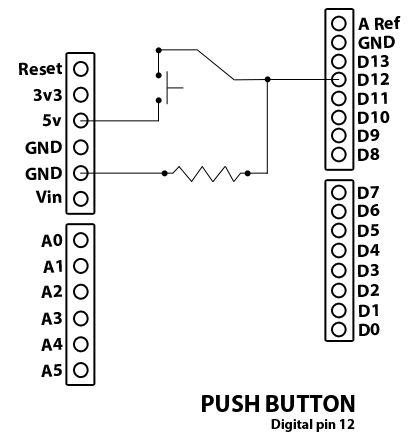
\includegraphics[width=\smfig]{\LocPushfig/pushbutton-conn.png}
\caption{Internal connection diagram for the pushbutton on the shield}
%\redcolor{connected on pin no. D12}}
\label{fig:pushbuttonconn}
\end{figure}


\begin{figure}
  \centering
  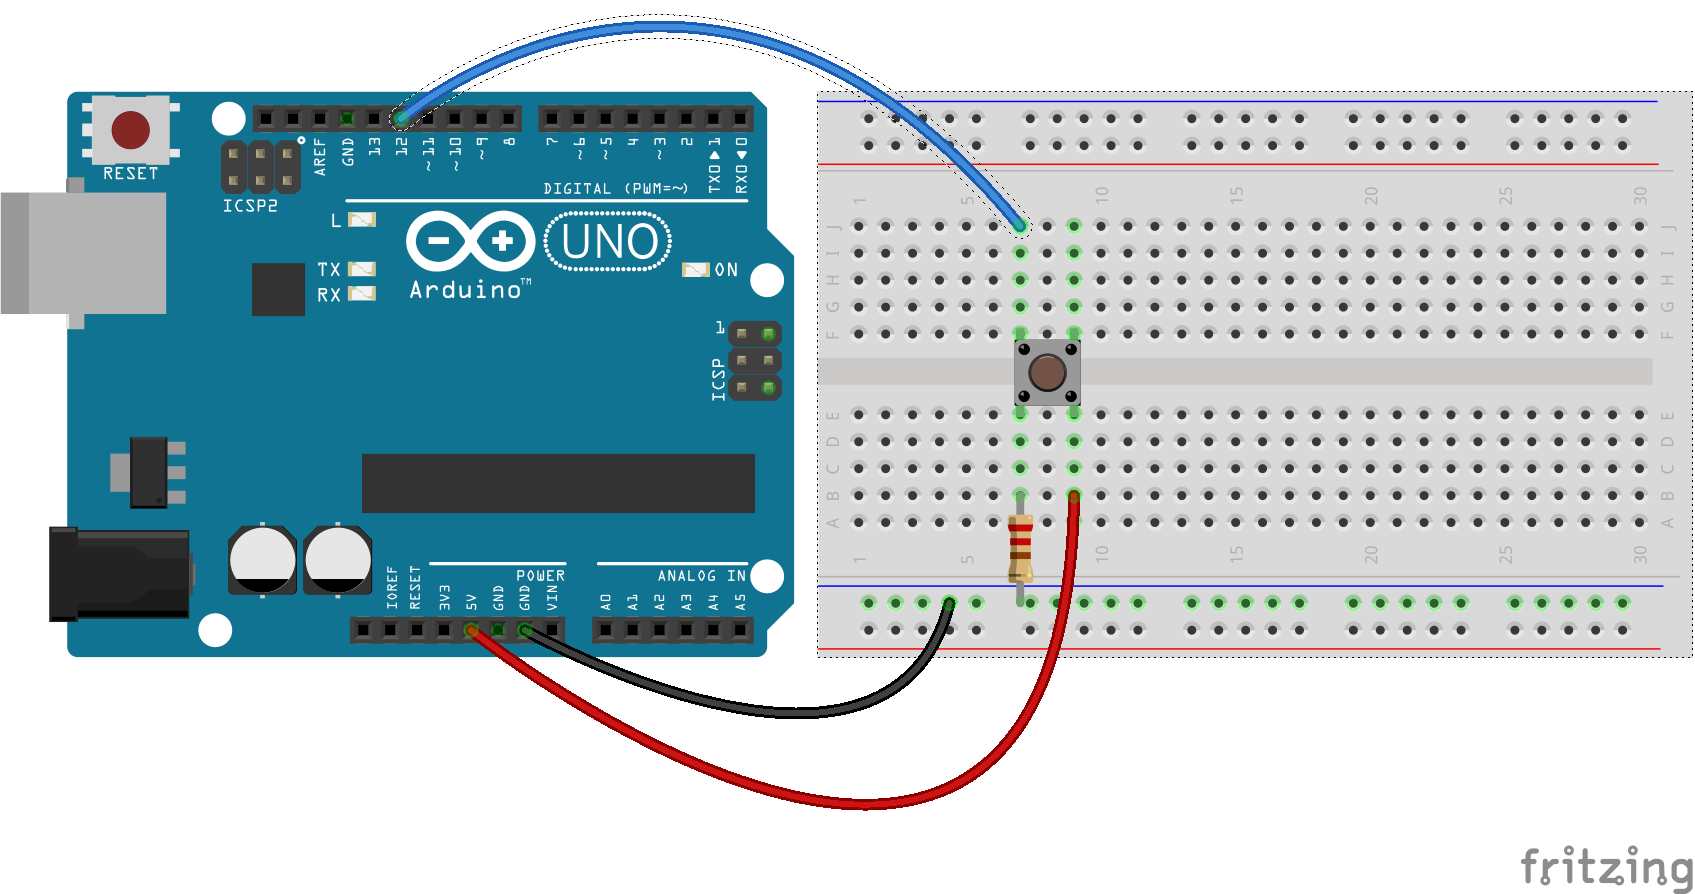
\includegraphics[width=\textwidth]{\LocPushfig/switch.png}
  \caption{A pushbutton to read its status with Arduino Uno using a breadboard}
  %\redcolor{connected on pin no. D12}}
  \label{fig:switch-bread}
\end{figure}

\section{Connecting a pushbutton with \arduino\ using a breadboard}
This section is useful for those who either don't have a shield or don't want to use the shield
for performing the experiments given in this chapter. 

A breadboard is a device for holding the components of a circuit and connecting 
them together. We can build an electronic circuit on a breadboard without doing any 
soldering. To know more about the breadboard and other electronic components, 
one should watch the Spoken Tutorials on Arduino as published on
{\tt https://spoken-tutorial.org/}. Ideally, one should go through all the
tutorials labeled as Basic. However, we strongly recommend the readers should
watch the fifth and sixth tutorials, i.e., {\tt First Arduino Program} and 
{\tt Arduino with Tricolor LED and Push button}.

In case you have a pushbutton, and you want to connect it with \arduino\ on a breadboard, 
please refer to \figref{fig:switch-bread}. The connections given in this figure can be used to 
read the status of a pushbutton. As shown in \figref{fig:switch-bread}, 
there are three different wires - red, black, and blue. The red wire is used to connect 5V on 
\arduino\ and one leg of the pushbutton. The black wire connects to one long vertical row on 
the side of the breadboard to provide access to the ground (GND) on \arduino. 
The blue wire goes from digital pin 12 to one leg of the pushbutton on another side. 
That same leg of the pushbutton connects through a pull-down resistor to GND on \arduino. 
When the pushbutton is open (unpressed), there is no connection between the two legs of the pushbutton, 
so the pin is connected to the ground (through the pull-down resistor), and we read a LOW on
digital pin 12. When the pushbutton is closed (pressed), it makes a connection between its two legs, 
connecting the pin to 5V so that we read a HIGH on digital pin 12. 

\begin{figure}
  \centering
  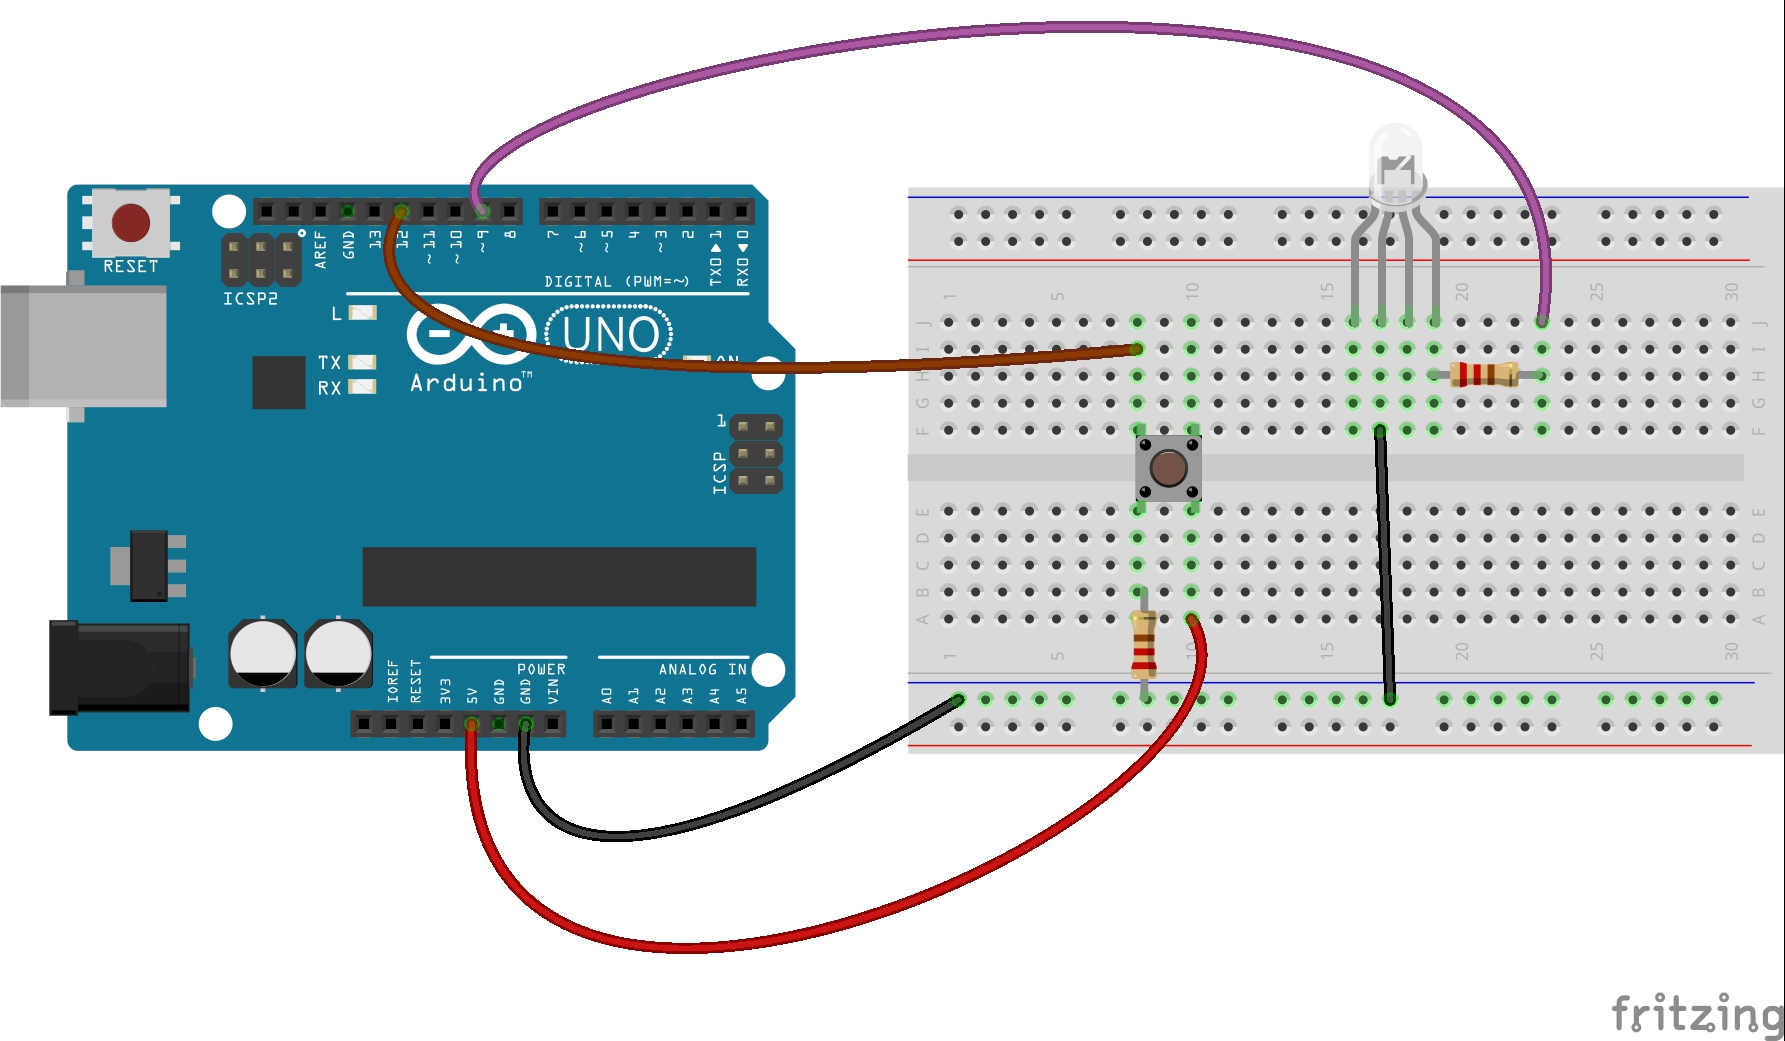
\includegraphics[width=\textwidth]{\LocPushfig/switch-led-dark-color-wires.jpg}
  \caption{A pushbutton to control an LED with Arduino Uno using a breadboard}
  %\redcolor{connected on pin no. D12}}
  \label{fig:switch-led}
\end{figure}
The connections shown in \figref{fig:switch-led} can be used to control an RGB LED, 
depending on the status of the pushbutton. As shown in \figref{fig:switch-led}, digital
pin 9 on \arduino\ is connected to the rightmost leg of the RGB LED. Rest of the connections
are same as that in \figref{fig:switch-bread}. 

\section{Reading the pushbutton status from the Arduino IDE}
\subsection{Reading the pushbutton status}
In this section, we shall describe an experiment that will help 
to read the status of a pushbutton through Arduino IDE. 
Later, we shall change the state of an LED depending on the status of the pushbutton. The shield has to be attached to the \arduino\ board
before doing these experiments and the \arduino\ needs to be connected to the computer 
with a USB cable, as shown in \figref{arduino}. The reader should go through the
instructions given in \secref{sec:ard-start} before getting started.
\begin{enumerate}
\item In the first experiment, we shall simply read the status of the
  pushbutton. Recall that it is a normally open type of switch. So, in
  an unpressed state, the logic read will be ``0'', corresponding to
  0V. And, when the user presses the pushbutton, the reading would be
  ``1'', corresponding to 5V. The code for this experiment is given in
  \ardref{ard:push-100}. In the initialization part of the code, we
  assign the sensor pin to be read, 12 in this case, to a variable for
  ease. Next, we initialize the port for serial port communication at
  data rate of 115200 bits per second and declare the digital pin 12 as an 
  input pin using the command {\tt pinMode}.  After initialization, 
  we start reading the status of the pushbutton using the following command:
  \lstinputlisting[firstline=7,lastline=7]
  {\LocPushardcode/push-button-status/push-button-status.ino}

  Note that the input argument to this command is the digital pin 12
  corresponding to the pin to which the pushbutton is connected.  After
  acquiring the values, we print them using,
  \lstinputlisting[firstline=8,lastline=8]
  {\LocPushardcode/push-button-status/push-button-status.ino} We
  repeat this read and print process 50 times by putting the
  commands in a {\tt for} loop. While running this experiment, the readers must press
  and release the pushbutton and observe the values being printed on the
  {\tt Serial Monitor} of Arduino IDE.

\item In the second experiment, we shall control the power given to an
  LED as per the status of the pushbutton. The code for this
  experiment is given in \ardref{ard:push-200}. This experiment can be
  taken as a step further to the previous one. We declare the LED pin
  to be controlled as an output pin by,
  \lstinputlisting[firstline=7,lastline=7]
  {\LocPushardcode/led-push-button/led-push-button.ino} Next, we read
  the pusbhutton value from digital pin 12. If the value is ``1'',
  we turn on the LED at pin 9 else we turn it off. The
  condition check is performed using {\tt if else} statements. We run
  these commands for 50 iterations. While running this experiment, the readers 
  must press and release the pushbutton. Accordingly, they can observe whether 
  the LED glows when the pushbutton is pressed. 
  %  \redcolor{Serial monitor}.
\end{enumerate}

\subsection{Arduino Code}
\lstset{style=mystyle}
\label{sec:push-arduino-code}
\addtocontents{ard}{\protect\addvspace{\codclr}}

\begin{ardcode}
  \acaption{Read the status of the pushbutton and display it on the
  Serial Monitor}{Read the status of the pushbutton and display it on
    the Serial Monitor.  Available at
    \LocPushardbrief{push-button-status/push-button-status.ino}.}
\label{ard:push-100}
\lstinputlisting{\LocPushardcode/push-button-status/push-button-status.ino}
\end{ardcode}

\begin{ardcode}
  \acaption{Turning the LED on or off depending on the pushbutton}
  {Turning the LED on or off depending on the pushbutton.  Available
    at \LocPushardbrief{led-push-button/led-push-button.ino}.}
\label{ard:push-200}
\lstinputlisting{\LocPushardcode/led-push-button/led-push-button.ino}
\end{ardcode}


